% !TeX spellcheck = cs_CZ
{\tikzset{external/prefix={tikz/FYZI/}}
 \tikzset{external/figure name/.add={ch37_}{}}
%=========================== Kapitola: Kvantové chování ===========================================
\chapter{Kvantové chování}\label{fyz:IchapXXXVII}
\minitoc
\section{Mechanika atomů}\label{fyz:IchapXXXVIIsecI}
\section{Experiment s kulkami}\label{fyz:IchapXXXVIIsecII}
\section{Experiment s vlnami}\label{fyz:IchapXXXVIIsecIII}
\section{Experiment s elektrony}\label{fyz:IchapXXXVIIsecIV}
\section{Interference elektronových vln}\label{fyz:IchapXXXVIIsecV}
\section{Sledování elektronů}\label{fyz:IchapXXXVIIsecVI}
\section{Základní principy kvantové mechaniky}\label{fyz:IchapXXXVIIsecVII}
\section{Princip neurčitosti}\label{fyz:IchapXXXVIIsecVIII}
\section{Příklady a cvičení}\label{fyz:IchapXXXVIIsecIX}

  \begin{figure}[ht!] %\ref{fyz:fig426}
    \centering
    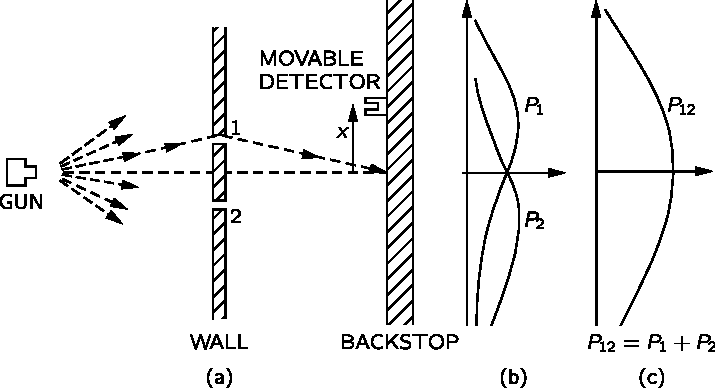
\includegraphics[width=0.6\linewidth]{fyz_fig426.pdf}
    \caption{
             (\cite[s.~697]{Feynman01})}
    \label{fyz:fig426}
  \end{figure}

  \begin{figure}[ht!] %\ref{fyz:fig427}
    \centering
    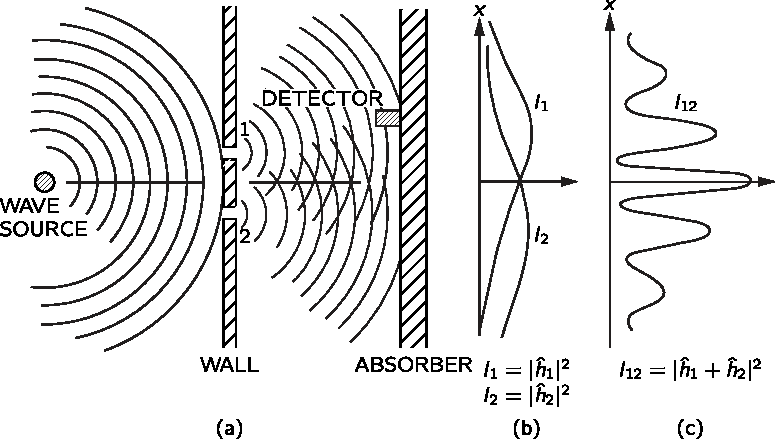
\includegraphics[width=0.6\linewidth]{fyz_fig427.pdf}
    \caption{
             (\cite[s.~697]{Feynman01})}
    \label{fyz:fig427}
  \end{figure}
  
  \begin{figure}[ht!] %\ref{fyz:fig428}
    \centering
    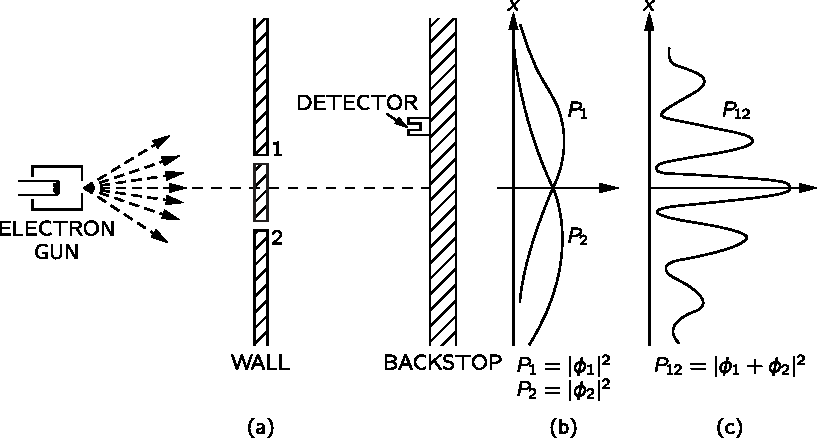
\includegraphics[width=0.6\linewidth]{fyz_fig428.pdf}
    \caption{
             (\cite[s.~697]{Feynman01})}
    \label{fyz:fig428}
  \end{figure}

  \begin{figure}[ht!] %\ref{fyz:fig429}
    \centering
    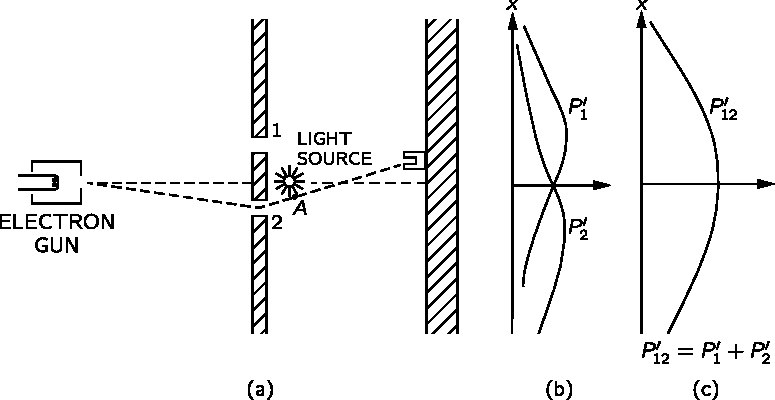
\includegraphics[width=0.6\linewidth]{fyz_fig429.pdf}
    \caption{
             (\cite[s.~697]{Feynman01})}
    \label{fyz:fig429}
  \end{figure}

  \begin{figure}[ht!] %\ref{fyz:fig430}
    \centering
    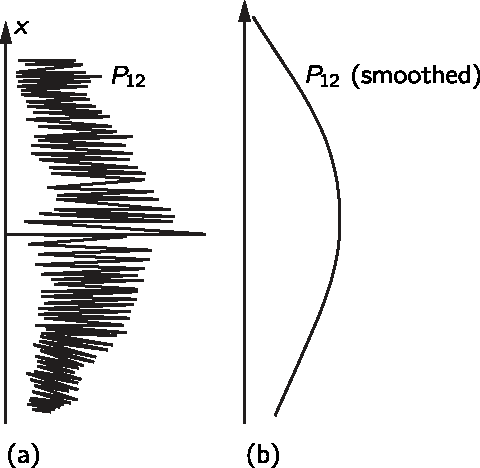
\includegraphics[width=0.6\linewidth]{fyz_fig430.pdf}
    \caption{
             (\cite[s.~697]{Feynman01})}
    \label{fyz:fig430}
  \end{figure}

  \begin{figure}[ht!] %\ref{fyz:fig431}
    \centering
    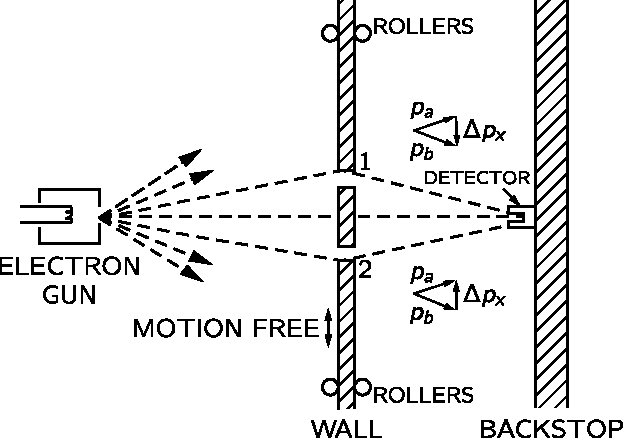
\includegraphics[width=0.6\linewidth]{fyz_fig431.pdf}
    \caption{
             (\cite[s.~697]{Feynman01})}
    \label{fyz:fig431}
  \end{figure}
  
  
} %tikzset
%~~~~~~~~~~~~~~~~~~~~~~~~~~~~~~~~~~~~~~~~~~~~~~~~~~~~~~~~~~~~~~~~~~~~~~~~~~~~~~~~~~~~~~~~~~~~~~~~~~
\printbibliography[title={Seznam literatury}, heading=subbibliography]
\addcontentsline{toc}{section}{Seznam literatury}